\documentclass[leqno]{article}
% Shared QBT/Soln pack preamble for resources.danieljsmith.org.
\usepackage{graphicx}
\usepackage{dsfont}
\usepackage{mathtools}
\usepackage{amssymb}
\usepackage{amsmath}
\usepackage{mleftright}
\usepackage{amsthm}
\usepackage{float}
\usepackage{ragged2e}
\usepackage{tensor}
\usepackage{fancyhdr}
\usepackage{empheq}
\usepackage[most]{tcolorbox}
\usepackage{enumitem}
\usepackage{dirtytalk}
\usepackage{marginnote}
\usepackage{microtype}
\usepackage[
  a4paper,
  left=0.8in,
  right=1in,
  top=1in,
  bottom=0.5in,
  headheight=14pt,
  headsep=0.4in
]{geometry}
\setlength{\parindent}{0cm}

% TikZ / PGFPlots
\usepackage{pgfplots}
\pgfplotsset{compat=1.18}
\usepgfplotslibrary{fillbetween, polar}
\usetikzlibrary{calc, positioning}
\usetikzlibrary{angles, quotes}
\usetikzlibrary{arrows.meta}
\usetikzlibrary{decorations.pathreplacing, decorations.markings}
\usetikzlibrary{patterns}
\usetikzlibrary{intersections}

% Links and contents. The contents follow the TMUA papers: compact entries,
% no dot leaders, and each question's mark total in grey after its label.
\usepackage{tocloft}
\tocloftpagestyle{fancy}
\setlength{\cftbeforesubsecskip}{2pt}
\setlength{\cftsubsecindent}{1.5em}
\setlength{\cftsubsecnumwidth}{0pt}
\renewcommand{\cftsubsecfont}{\small\color{black}}
\renewcommand{\cftsubsecpagefont}{\small\color{black}}
\renewcommand{\cftsubsecleader}{\hfill}
\usepackage[colorlinks=true,linkcolor=black,citecolor=magenta,urlcolor=black]{hyperref}%
\urlstyle{same}

% Pack macros
% \marks also adds its value to the current question's total in the .aux
% file, so the contents show each total from the second pass. The write
% happens at shipout, so a box typeset more than once counts once. The
% pack's mark total for the contents-page title is summed the same way.
\makeatletter
\newcount\djs@totalmarks
\newcommand{\djsAddMarks}[2]{%
  \global\advance\djs@totalmarks#2\relax
  \@ifundefined{djs@marks@#1}%
    {\expandafter\xdef\csname djs@marks@#1\endcsname{#2}}%
    {\expandafter\xdef\csname djs@marks@#1\endcsname
      {\the\numexpr\csname djs@marks@#1\endcsname+#2\relax}}}
\RenewDocumentCommand{\marks}{o m}{%
  \protected@write\@auxout{}{\string\djsAddMarks{\number\value{enumi}}{#2}}%
  \IfValueTF{#1}%
    {\marginnote{\raggedright\textbf{[#2]}}[#1]}%
    {\marginnote{\raggedright\textbf{[#2]}}}%
}
\makeatother

\newcommand{\vspacerule}[2]{%
  \par\vspace*{#1}%
  \noindent\hrulefill\par
  \vspace*{#2}%
}

\definecolor{scarlet}{RGB}{205, 40, 75}
% Site colours for the contents-page title: the accent, the rule colour, a
% stronger rule colour for the path separator, and the muted text colour.
\definecolor{djsBurgundy}{RGB}{118, 59, 67}
\definecolor{djsHairline}{RGB}{216, 213, 205}
\definecolor{djsSlash}{RGB}{170, 166, 158}
\definecolor{djsMuted}{RGB}{96, 101, 106}

% Worked-solution box, adapted from the TMUA worked-solutions box. A white breakable box with a left scarlet rule and no surrounding
% frame or tint. A part that breaks fills the rest of its page, so the rule
% runs to the bottom margin; the unbroken or last part ends in a short
% horizontal foot rule so a solution visibly stops. Unlike the TMUA box there
% is no answer label. The box does not grow to the left, so the rule sits at
% the text edge; growing to the right keeps the usable line width close to the
% old tcolorbox Solution box.
% Spacing inside the box: paragraphs are 6pt apart, so source blank lines show
% (solutions put one after each display and none between a lead-in and its
% display). Every display gets 6pt above and 10pt below, whatever the length
% of its lead-in line; align rows are spread by an 8pt \jot; solution parts
% are 14pt apart and sub-parts 8pt; \left and \right space like ordinary
% brackets (mleftright); no single line is stranded at a page break; and
% neither the Solution label nor the line before a list ends a page. No
% skip can shrink, so full pages are not squeezed.
\newtcolorbox{djsSolution}{%
  enhanced, breakable, frame hidden, sharp corners, colback=white,
  height fixed for=first and middle, height fill,
  extras unbroken and last={natural height},
  borderline west={2.2pt}{0pt}{scarlet},
  left=11pt, right=0pt, top=5pt, bottom=13pt,
  before skip=13pt, after skip=4pt,
  grow to right by=10mm,
  overlay unbroken and last={%
    \fill[scarlet] (frame.south west)
      rectangle ([xshift=3.5cm, yshift=2.2pt]frame.south west);},
  before upper={{\color{scarlet}\bfseries Solution}\par\nobreak\vspace{4pt}%
    \setlength{\parskip}{6pt plus 2pt}%
    \setlength{\abovedisplayskip}{6pt plus 2pt}%
    \setlength{\abovedisplayshortskip}{6pt plus 2pt}%
    \setlength{\belowdisplayskip}{10pt plus 2pt}%
    \setlength{\belowdisplayshortskip}{10pt plus 2pt}%
    \setlength{\jot}{8pt}%
    \setlist{parsep=6pt plus 2pt, topsep=6pt plus 2pt, beginpenalty=10000}%
    \setlist[enumerate,1]{itemsep=14pt plus 2pt}%
    \setlist[enumerate,2]{itemsep=8pt plus 2pt}%
    \mleftright
    \clubpenalty=10000 \widowpenalty=10000 \displaywidowpenalty=10000\relax}}

% Optional smaller figure inside a solution box. \scalebox shrinks node text
% with the drawing. Not applied to existing figures.
\newcommand{\SolnFigureScale}{0.85}
\newsavebox{\djsSolnFigureBox}
\newenvironment{djsSolutionFigure}
  {\par\vspace{4pt}\begin{center}\begin{lrbox}{\djsSolnFigureBox}}
  {\end{lrbox}\scalebox{\SolnFigureScale}{\usebox{\djsSolnFigureBox}}%
   \end{center}\vspace{2pt}\par}

\newcommand{\cxl}[2]{%
  \tikz[baseline=(X.base)]{%
    \node[inner sep=0pt, outer sep=0pt, text=#1] (X) {$#2$};
    \draw[#1, line width=0.4pt] (X.south west)--(X.north east);
  }%
}

% Page-style hook run at the contents page and each question's opening page.
% A no-op for QBT packs; \djsSolnHeader points it at the fancy header.
\newcommand{\djsQuestionPageStyle}{}

% A contents entry: "Question N" in a box wide enough for two digits, so the
% mark totals line up, then the total in grey. Bookmarks keep "Question N".
\makeatletter
\newlength{\djsTocLabelWidth}
\newcommand{\djsTocMarks}[1]{%
  \@ifundefined{djs@marks@#1}{}{%
    {\footnotesize\itshape\color{black!45}%
     \csname djs@marks@#1\endcsname~mark%
     \ifnum\csname djs@marks@#1\endcsname=1 \else s\fi}}}
\newcommand{\djsTocEntry}[1]{%
  \texorpdfstring
    {\settowidth{\djsTocLabelWidth}{Question 00}%
     \makebox[\dimexpr\djsTocLabelWidth+0.9em\relax][l]{Question #1}%
     \djsTocMarks{#1}}%
    {Question #1}}
\makeatother

% The question count for the contents-page title is written to the .aux at
% the end of the document, so it also appears from the second pass.
\newcounter{djsQuestions}
\newcommand{\questionitem}{%
  \djsQuestionPageStyle
  \item\phantomsection
  \stepcounter{djsQuestions}%
  \addcontentsline{toc}{subsection}{\protect\djsTocEntry{\number\value{enumi}}}%
}
\makeatletter
\newcommand{\djsSetQuestionCount}[1]{\gdef\djs@questioncount{#1}}
\AtEndDocument{\immediate\write\@auxout
  {\string\djsSetQuestionCount{\number\value{djsQuestions}}}}
\makeatother

\renewcommand{\contentsname}{Questions}

% \djsPackHeader[<link content tag>]{<left header>}; the tag says which
% document a click on the header link came from.
\newcommand{\djsPackHeader}[2][questions]{%
  \pagestyle{fancy}%
  \fancyhead{}%
  \fancyfoot{}%
  \renewcommand{\headrulewidth}{0.9pt}%
  \lhead{#2}%
  \chead{}%
  \rhead{\href{https://danieljsmith.org/?utm_source=pdf&utm_campaign=further-maths&utm_content=#1}{danieljsmith.org}}%
}

% The header's topic is also the contents-page title, under which a label
% says which booklet this is.
\newcommand{\djsPackTitle}{}
\newcommand{\djsBookletLabel}{}
\newcommand{\djsQbtHeader}[1]{%
  \djsPackHeader{#1}%
  \renewcommand{\djsPackTitle}{#1}%
  \renewcommand{\djsBookletLabel}{Questions by topic}%
}

% The colophon at the foot of page one, independent of the page style: the
% contents-page title's hairline led by a short scarlet rule, then the date on
% the left and a link to the site on the right, all inside the bottom margin.
% Its sizes are fixed, so it matches the TMUA papers' colophon. The document
% supplies the date; recompiling never changes it.
\makeatletter
\newcommand{\djsLastUpdated}[1]{%
  \AtBeginDocument{\AddToHookNext{shipout/foreground}{\djs@colophon{#1}}}}
\newcommand{\djs@colophon}[1]{%
  \put(0.8in,-\dimexpr\paperheight-0.47in\relax){%
    \makebox[0pt][l]{\color{djsHairline}%
      \rule[0.9pt]{\dimexpr\paperwidth-1.8in\relax}{0.6pt}}%
    \makebox[0pt][l]{\color{scarlet}\rule{3.5cm}{2.2pt}}}%
  \put(0.8in,-\dimexpr\paperheight-0.32in\relax){\makebox[0pt][l]{%
    \fontsize{9}{11}\selectfont Last updated #1}}%
  \put(\dimexpr\paperwidth-1in\relax,-\dimexpr\paperheight-0.32in\relax){%
    \makebox[0pt][r]{\fontsize{7}{8.5}\selectfont\color{djsMuted}%
      Latest version at \href{https://resources.danieljsmith.org/}%
        {\color{black}resources.danieljsmith.org}}}}
\makeatother

% Solutions packs show the header only on the contents page and each
% question's opening page, so it never appears part-way through a solution.
% \thispagestyle marks the next page shipped out, which is the question's
% page because every solution question starts after a \newpage.
\newcommand{\djsSolnHeader}[1]{%
  \djsPackHeader[solutions]{\textit{Solutions} - #1}%
  \pagestyle{empty}%
  \renewcommand{\djsQuestionPageStyle}{\thispagestyle{fancy}}%
  \renewcommand{\djsPackTitle}{#1}%
  \renewcommand{\djsBookletLabel}{Worked solutions}%
}

% \djsSitePath{<strand>}{<topic>}, called once after the header, names where
% the pack sits on the site; the contents-page title prints it above the pack
% title, e.g. CORE PURE / FURTHER CALCULUS. Without it the line is left out.
\makeatletter
\newif\ifdjs@sitepath
\newcommand{\djs@strand}{}
\newcommand{\djs@section}{}
\newcommand{\djsSitePath}[2]{%
  \djs@sitepathtrue
  \renewcommand{\djs@strand}{#1}%
  \renewcommand{\djs@section}{#2}%
}
\makeatother

% Further Mechanics packs call \djsMechanicsPack in their preamble, so that
% \djsFrontMatter prints the default value of g above the contents. The box
% keeps its own space above it (before skip is the whole gap below the title,
% not an addition to it). Without the box, \djsGravityNote is just extra space
% before the contents heading, bringing the gap above it close to the gap
% between the box and the heading on Further Mechanics pages.
\newcommand{\djsGravityNote}{\vspace{14pt}}
\newcommand{\djsMechanicsPack}{%
  \renewcommand{\djsGravityNote}{%
    \begin{tcolorbox}[sharp corners, colback=white, colframe=black,
      boxrule=1pt, left=8pt, right=8pt, top=6pt, bottom=6pt,
      before skip=20pt]
    {\bfseries Instructions}\par\vspace{4pt}
    Unless a question states otherwise, take $g = 9.8\,\mathrm{m\,s^{-2}}$
    wherever a numerical value of $g$ is required. Solutions also give final
    answers for $g = 10\,\mathrm{m\,s^{-2}}$ where these differ.
    \end{tcolorbox}%
    \vspace{16pt}}%
}

% Contents-page title: the site path in spaced burgundy capitals, the pack
% title, a hairline led by a short scarlet rule (the solution box's foot rule),
% then the booklet label with the question and mark counts. The counts come
% from the .aux, so they appear from the second pass.
\makeatletter
\newsavebox{\djs@eyebrowbox}
\newcommand{\djs@caps}[1]{\textls[180]{\MakeUppercase{#1}}}
\newcommand{\djs@eyebrow}{%
  \color{djsBurgundy}\footnotesize\bfseries
  \djs@caps{\djs@strand}%
  {\color{djsSlash}\hspace{0.55em}/\hspace{0.55em}}%
  \djs@caps{\djs@section}}
\newcommand{\djs@dot}{\hspace{0.45em}\textperiodcentered\hspace{0.45em}}
\newcommand{\djs@counts}{%
  \@ifundefined{djs@questioncount}{}{%
    \djs@questioncount~question\ifnum\djs@questioncount=1 \else s\fi
    \ifnum\djs@totalmarks>0
      \djs@dot\the\djs@totalmarks~mark\ifnum\djs@totalmarks=1 \else s\fi
    \fi}}
\newcommand{\djsContentsTitle}{%
  \ifdjs@sitepath
    \sbox\djs@eyebrowbox{\djs@eyebrow}%
    \ifdim\wd\djs@eyebrowbox>\linewidth
      \@latex@warning@no@line{The \string\djsSitePath\space line is wider
        than the text, so it wraps. Shorten its topic}%
    \fi
    {\raggedright\djs@eyebrow\par}%
    \vspace{7pt}%
  \fi
  {\raggedright\fontsize{24.88}{28}\selectfont\djsPackTitle\par}%
  \vspace{9pt}%
  \noindent\makebox[0pt][l]{\color{djsHairline}\rule[0.9pt]{\linewidth}{0.6pt}}%
  {\color{scarlet}\rule{3.5cm}{2.2pt}}\par
  \vspace{5pt}%
  {\small\color{djsMuted}\djsBookletLabel\hfill\djs@counts\par}%
  \vspace{8pt}%
}
\makeatother

\newcommand{\djsFrontMatter}{%
  \djsQuestionPageStyle
  \vspace*{6pt}%
  \djsContentsTitle
  \djsGravityNote
  \tableofcontents
  \newpage
}


\djsQbtHeader{Centre of Mass of Laminae by Integration}
\djsSitePath{Further Mechanics}{Centre of Mass}
\djsMechanicsPack
\djsLastUpdated{14 October 2026}

\begin{document}
\djsFrontMatter
\begin{enumerate}[
  label=\textbf{\arabic*.},
  leftmargin=*,
  topsep=0pt,
  partopsep=0pt,
  parsep=0pt
]

% ---- Question 1 ----
\questionitem
% [Source: _QBT__Centre_of_Mass_of_Laminae_by_Integration, Q1]

\begin{figure}[H]
    \centering
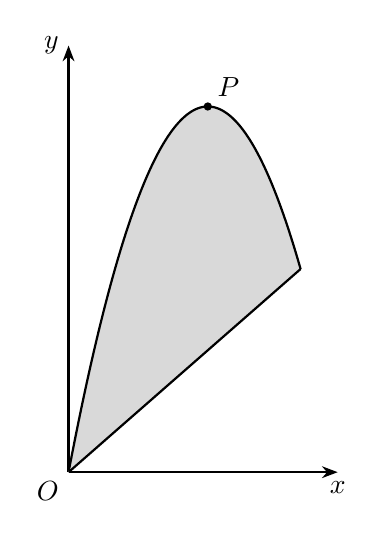
\begin{tikzpicture}
\def\coeff{6}
\def\slope{1}
\pgfmathsetmacro{\rightbound}{\coeff-\slope}
\pgfmathsetmacro{\px}{\coeff/2}
\pgfmathsetmacro{\py}{\coeff*\px-\px^2}
\pgfmathsetmacro{\xmax}{\rightbound+0.8}
\pgfmathsetmacro{\ymax}{\py+1.5}
\begin{axis}[
  width=5cm, height=7cm,
  axis lines=left,
  axis line style={thick, black, -{Stealth[length=2mm]}},
  xlabel={$x$}, ylabel={$y$},
  xmin=0, xmax=\xmax, ymin=0, ymax=\ymax,
  xtick=\empty, ytick=\empty,
  clip=true, clip mode=individual,
  every axis x label/.style={at={(ticklabel* cs:1)}, anchor=north},
  every axis y label/.style={at={(ticklabel* cs:1)}, anchor=east}
]
\addplot[draw=none, name path=upper, domain=0:\rightbound, samples=150] {\coeff*x-x^2};
\addplot[draw=none, name path=lower, domain=0:\rightbound, samples=2] {\slope*x};
\addplot[gray!30] fill between[of=upper and lower];
\addplot[thick, black, domain=0:\rightbound, samples=150] {\coeff*x-x^2};
\addplot[thick, black, domain=0:\rightbound, samples=2] {\slope*x};
\coordinate (P) at (axis cs:\px,\py);
\fill[black] (P) circle (1.5pt);
\node[above right] at (P) {$P$};
\node[below left] at (axis cs:0,0) {$O$};
\end{axis}
\end{tikzpicture}
\end{figure}


A uniform lamina occupies the region enclosed by the curve $y=6x-x^2$ and the straight line $y=x$. \\
The unit of length on each axis is one centimetre. \\
The diagram above shows the lamina and the point $P(3,9)$ at the maximum of the curve. \\
\begin{enumerate}[label=\textbf{(\alph*)}]
\item Find the area of the lamina and use integration to find the coordinates of its centre of mass. Give your answers in exact form. \marks{5} \\
\item The lamina is freely suspended from $P$ and hangs in equilibrium. \\
Find the acute angle between the vertical and the straight edge of the lamina, giving your answer to the nearest degree. \marks{3} \\
\end{enumerate}

\newpage

% ---- Question 2 ----
\questionitem
% [Source: _QBT__Centre_of_Mass_of_Laminae_by_Integration, Q2]

\begin{figure}[H]
    \centering
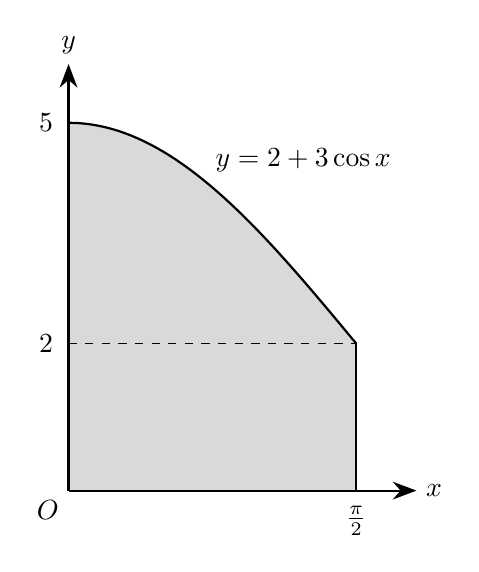
\begin{tikzpicture}
\def\baseheight{2}
\def\amplitude{3}
\pgfmathsetmacro{\rightbound}{pi/2}
\begin{axis}[
  width=6cm, height=7cm,
  axis lines=left,
  axis line style={thick, -{Stealth[length=3mm]}},
  xmin=0, xmax=1.9, ymin=0, ymax=5.8,
  xlabel={$x$}, ylabel={$y$},
  xtick={\rightbound}, xticklabels={$\frac{\pi}{2}$},
  ytick={2,5},
  tick style={draw=none},
  every axis x label/.style={at={(rel axis cs:1,0)},anchor=west},
  every axis y label/.style={at={(rel axis cs:0,1)},anchor=south},
  axis on top,
  clip=true,
  clip mode=individual
]
\addplot[draw=none, fill=gray!30, domain=0:\rightbound, samples=150] {\baseheight+\amplitude*cos(deg(x))} \closedcycle;
\addplot[thick, black, domain=0:\rightbound, samples=150] {\baseheight+\amplitude*cos(deg(x))};
\draw[thick, black] (axis cs:\rightbound,0) -- (axis cs:\rightbound,\baseheight);
\draw[dashed, black] (axis cs:0,\baseheight) -- (axis cs:\rightbound,\baseheight);
\node[above right] at (axis cs:0.75,{\baseheight+\amplitude*cos(deg(0.75))}) {$y=2+3\cos x$};
\node[below left] at (axis cs:0,0) {$O$};
\end{axis}
\end{tikzpicture}
\end{figure}


A uniform lamina $L$ is cut to form a decorative panel. \\
It occupies the region bounded by the curve $y=2+3\cos x$, the $x$-axis and the vertical lines $x=0$ and $x=\frac{\pi}{2}$, as shown in the diagram above. \\
Its centre of mass is $(\bar{x},\bar{y})$. \\

\begin{enumerate}[label=\textbf{(\alph*)}]
  \item Using integration, show that
  \[
  \bar{x}=\dfrac{\pi^2+6\pi-12}{4(\pi+3)}
  \] \marks[-30pt]{2}
  \item Find the exact value of $\bar{y}$. Hence show, without using decimal approximations, that the centre of mass lies above the line $y=2$. \marks{3} \\
\end{enumerate}

\newpage

% ---- Question 3 ----
\questionitem
% [Source: _QBT__Centre_of_Mass_of_Laminae_by_Integration, Q3]

\begin{figure}[H]
    \centering
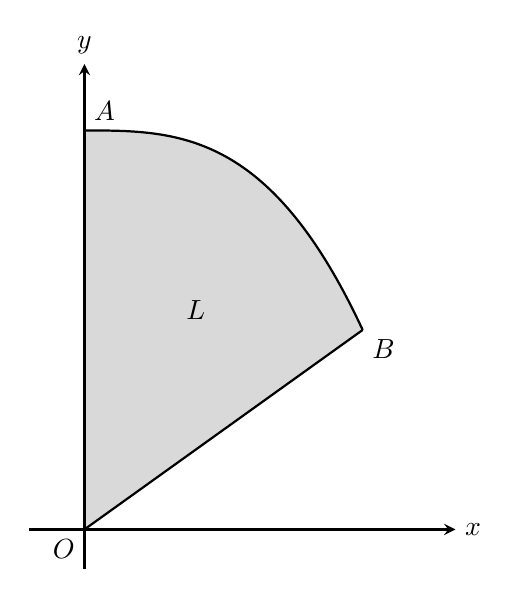
\begin{tikzpicture}
\def\xb{3}
\def\height{6}
\def\denom{9}
\pgfmathsetmacro{\yb}{\height-\xb^3/\denom}
\begin{axis}[
axis lines=center,
axis on top,
xlabel={$x$}, ylabel={$y$},
xmin=-0.6, xmax=4,
ymin=-0.6, ymax=7,
xtick=\empty, ytick=\empty,
width=7cm, height=8cm,
clip=true,
axis line style={thick, black},
every axis x label/.style={at={(ticklabel* cs:1)}, anchor=west},
every axis y label/.style={at={(ticklabel* cs:1)}, anchor=south}
]
\addplot[draw=none, name path=upper, domain=0:\xb, samples=150] {\height-x^3/\denom};
\addplot[draw=none, name path=lower, domain=0:\xb, samples=2] {x};
\addplot[gray!30] fill between[of=upper and lower];
\addplot[thick, black, domain=0:\xb, samples=150] {\height-x^3/\denom};
\addplot[thick, black, domain=0:\xb, samples=2] {x};
\coordinate (O) at (axis cs:0,0);
\coordinate (A) at (axis cs:0,\height);
\coordinate (B) at (axis cs:\xb,\yb);
\draw[thick, black] (O)--(A);
\node[below left] at (O) {$O$};
\node[above right] at (A) {$A$};
\node[below right] at (B) {$B$};
\node at (axis cs:{0.4*\xb},{0.55*\height}) {$L$};
\end{axis}
\end{tikzpicture}
\end{figure}


The diagram above shows a region bounded by the $y$-axis, the straight line $y=x$ and the curve
\[
y=6-\dfrac{x^3}{9}
\] \\
The curve meets the $y$-axis at $A=(0,6)$ and meets the line $y=x$ at $B=(3,3)$. \\
The origin is $O$. \\

A uniform lamina $L$ occupies the shaded region $OAB$. \\
The unit of length on each axis is one centimetre, and its centre of mass has coordinates $(\bar{x},\bar{y})$. \\
\begin{enumerate}[label=\textbf{(\alph*)}]
\item Use integration to find the area of $L$ and show that
\[
\bar{y}=\dfrac{118}{35}
\] \marks[-30pt]{5}
\item The lamina is freely suspended from $B$ and hangs in equilibrium. Find the acute angle between the straight edge $OB$ and the downward vertical, giving your answer in degrees to one decimal place. \marks{8} \\
\end{enumerate}

\newpage

% ---- Question 4 ----
\questionitem
% [Source: _QBT__Centre_of_Mass_of_Laminae_by_Integration, Q4]

\begin{figure}[H]
    \centering
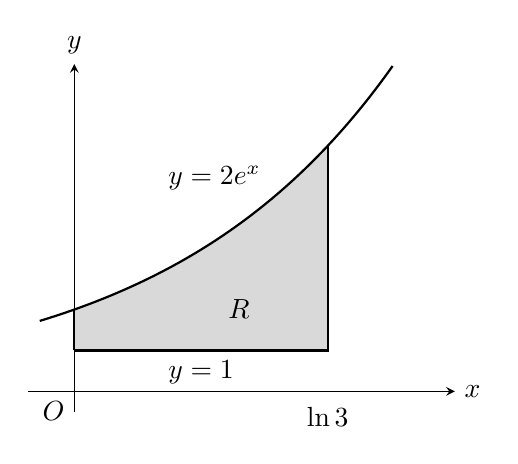
\begin{tikzpicture}
\def\coeff{2}
\def\base{1}
\pgfmathsetmacro{\rightx}{ln(3)}
\begin{axis}[
  width=7cm,height=6cm,
  axis lines=center,axis on top,
  xlabel={$x$},ylabel={$y$},
  xmin=-0.2,xmax=1.65,ymin=-0.5,ymax=8,
  xtick={\rightx},xticklabels={$\ln 3$},
  ytick=\empty,tick style={draw=none},
  clip=true,clip mode=individual,
  every axis x label/.style={at={(ticklabel* cs:1)},anchor=west},
  every axis y label/.style={at={(ticklabel* cs:1)},anchor=south}
]
\addplot[draw=none,name path=upper,domain=0:\rightx,samples=120] {\coeff*exp(x)};
\addplot[draw=none,name path=lower,domain=0:\rightx,samples=2] {\base};
\addplot[gray!30] fill between[of=upper and lower];
\addplot[thick,black,domain=-0.15:1.38,samples=150] {\coeff*exp(x)};
\draw[thick,black] (axis cs:0,\base) -- (axis cs:\rightx,\base) -- (axis cs:\rightx,{\coeff*exp(\rightx)});
\draw[thick,black] (axis cs:0,\base) -- (axis cs:0,\coeff);
\node[above left] at (axis cs:0.85,{\coeff*exp(0.85)}) {$y=2e^x$};
\node[below] at (axis cs:{\rightx/2},\base) {$y=1$};
\node at (axis cs:{0.65*\rightx},2) {$R$};
\node[below left] at (axis cs:0,0) {$O$};
\end{axis}
\end{tikzpicture}
\end{figure}


\begin{figure}[H]
    \centering
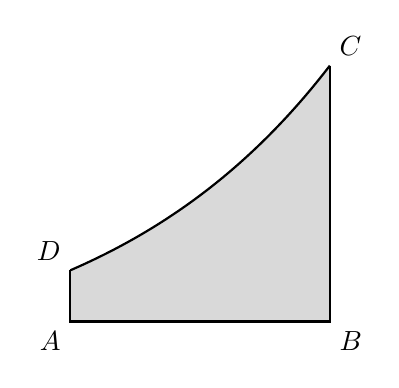
\begin{tikzpicture}[x=3cm,y=0.65cm]
\def\coeff{2}
\def\base{1}
\pgfmathsetmacro{\widthAB}{ln(3)}
\pgfmathsetmacro{\heightC}{\coeff*exp(\widthAB)}
\coordinate (A) at (0,\base);
\coordinate (B) at (\widthAB,\base);
\coordinate (C) at (\widthAB,\heightC);
\coordinate (D) at (0,\coeff);
\fill[gray!30] (A) -- (B) -- (C) -- plot[domain=\widthAB:0,samples=120] (\x,{\coeff*exp(\x)}) -- cycle;
\draw[thick,black] (D) -- (A) -- (B) -- (C);
\draw[thick,black] plot[domain=0:\widthAB,samples=120] (\x,{\coeff*exp(\x)});
\node[below left] at (A) {$A$};
\node[below right] at (B) {$B$};
\node[above right] at (C) {$C$};
\node[above left] at (D) {$D$};
\end{tikzpicture}
\end{figure}


The shaded region $R$ is bounded by the curve $y=2e^x$, the horizontal line $y=1$, the $y$-axis and the line $x=\ln 3$. \\
The unit of length on each axis is one metre. \\

A uniform lamina occupies $R$, and its centre of mass has coordinates $(\bar{x},\bar{y})$. \\
\begin{enumerate}[label=\textbf{(\alph*)}]
\item Use integration to find the area of $R$ and show that
\[
\bar{y}=\dfrac{16-\ln 3}{8-2\ln 3}
\] \marks[-30pt]{5}
\end{enumerate}
The second diagram above shows the same lamina, with vertices $A=(0,1)$, $B=(\ln 3,1)$, $C=(\ln 3,6)$ and $D=(0,2)$. \\

The lamina is freely suspended from $D$ and hangs in equilibrium. \\
Let $\theta$ be the angle between the directed segment from $D$ to $A$ and the downward vertical, where $0^\circ\leq\theta\leq180^\circ$. \\
\begin{enumerate}[label=\textbf{(\alph*)}, resume]
\item Use integration to find $\bar{x}$ in exact form. Hence find $\theta$, giving your answer to one decimal place. \marks{7} \\
\end{enumerate}

\newpage

% ---- Question 5 ----
\questionitem
% [Source: _QBT__Centre_of_Mass_of_Laminae_by_Integration, Q5]

A uniform lamina occupies the region bounded by the curve
\[
y=\dfrac{k}{x+1}
\] \\
the $x$-axis and the vertical lines $x=0$ and $x=3$, where $k$ is a positive constant. \\

\begin{enumerate}[label=\textbf{(\roman*)}]
  \item Find the exact $x$-coordinate of the centre of mass of the lamina. \marks{6} \\
  \item The centre of mass lies on the line $y=x$. \\
  Find the exact value of $k$ and hence the exact area of the lamina. \marks{5} \\
\end{enumerate}

\newpage

% ---- Question 6 ----
\questionitem
% [Source: _QBT__Centre_of_Mass_of_Laminae_by_Integration, Q6]

\begin{figure}[H]
    \centering
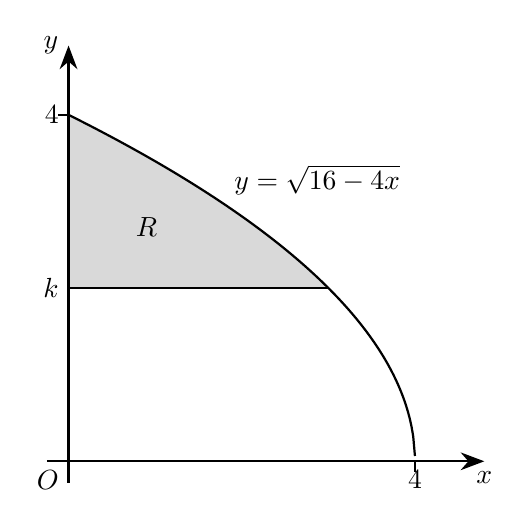
\begin{tikzpicture}[scale=1.1]
\def\height{4}
\def\coeff{4}
\def\kval{2}
\def\margin{0.8}
\def\ticklen{0.12}
\pgfmathsetmacro{\endx}{\height*\height/\coeff}
\pgfmathsetmacro{\cutx}{(\height*\height-\kval*\kval)/\coeff}
\coordinate (O) at (0,0);
\coordinate (Y) at (0,\height);
\coordinate (X) at (\endx,0);
\coordinate (K) at (0,\kval);
\coordinate (P) at (\cutx,\kval);
\coordinate (CLabel) at ({0.45*\endx},{sqrt(\height*\height-\coeff*0.45*\endx)});
\coordinate (RLabel) at ({0.3*\cutx},{\kval+0.35*(\height-\kval)});
\fill[gray!30] (K) -- (P) -- plot[domain=\cutx:0,samples=150] (\x,{sqrt(max(0,\height*\height-\coeff*\x))}) -- cycle;
\draw[thick,black,-{Stealth[length=3mm]}] (-0.25,0) -- ({\endx+\margin},0) node[below] {$x$};
\draw[thick,black,-{Stealth[length=3mm]}] (0,-0.25) -- (0,{\height+\margin}) node[left] {$y$};
\draw[thick,black,domain=0:\endx,samples=200] plot (\x,{sqrt(max(0,\height*\height-\coeff*\x))});
\draw[thick,black] (K) -- (P);
\draw[thick,black] ($(Y)+(-\ticklen,0)$) -- (Y);
\draw[thick,black] ($(X)+(0,-\ticklen)$) -- (X);
\node[below left] at (O) {$O$};
\node[left] at (Y) {$4$};
\node[below] at (X) {$4$};
\node[left] at (K) {$k$};
\node[above right] at (CLabel) {$y=\sqrt{16-4x}$};
\node at (RLabel) {$R$};
\end{tikzpicture}
\end{figure}


The shaded region $R$ is bounded by the curve $y=\sqrt{16-4x}$, the $y$-axis and the horizontal line $y=k$, where $0<k<4$. \\
A uniform lamina occupies $R$. \\
\begin{enumerate}[label=\textbf{(\alph*)}]
\item Using integration, determine the $y$-coordinate of the centre of mass of the lamina in terms of $k$. Simplify your expression fully. \marks{6} \\
\item The centre of mass lies on the line $y=3$. Find the exact value of $k$, explaining why any other root of your equation must be rejected. \marks{3} \\
\end{enumerate}

\newpage

% ---- Question 7 ----
\questionitem
% [Source: _QBT__Centre_of_Mass_of_Laminae_by_Integration, Q7]

A uniform lamina occupies the region between the curve $y=4e^{-x/2}$ and the line $y=1$, for $0\leq x\leq 2\ln 2$. \\
\begin{enumerate}[label=\textbf{(\roman*)}]
\item Using integration, find the exact area of this lamina and the exact $y$-coordinate of its centre of mass. \marks{7} \\
\end{enumerate}

\begin{figure}[H]
    \centering
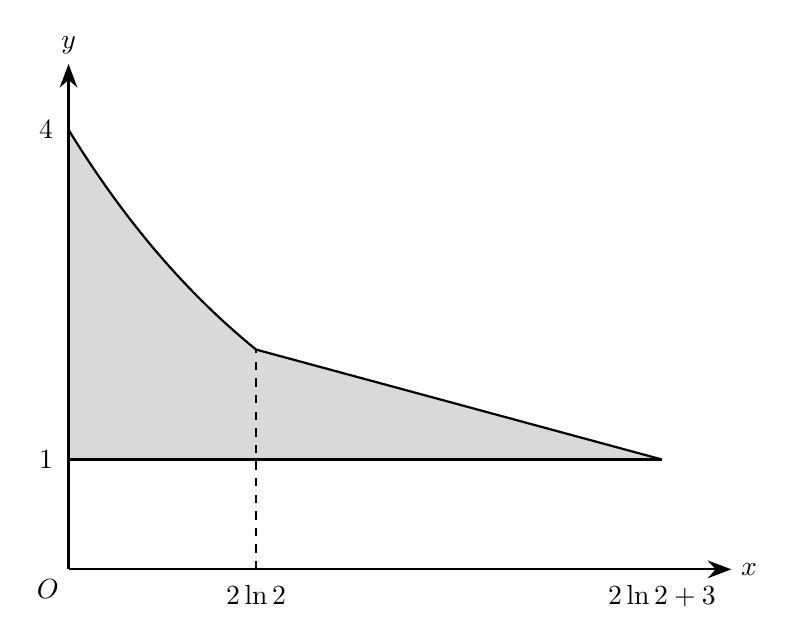
\begin{tikzpicture}
\def\height{4}
\def\baseline{1}
\def\extension{3}
\pgfmathsetmacro{\joinx}{2*ln(2)}
\pgfmathsetmacro{\joiny}{\height*exp(-\joinx/2)}
\pgfmathsetmacro{\endx}{\joinx+\extension}
\begin{axis}[
  width=10cm, height=8cm,
  axis lines=left,
  axis line style={thick, black, -{Stealth[length=3mm]}},
  xlabel={$x$}, ylabel={$y$},
  xmin=0, xmax=4.9, ymin=0, ymax=4.6,
  xtick={\joinx,\endx},
  xticklabels={$2\ln 2$,$2\ln 2+3$},
  ytick={1,4},
  tick style={draw=none},
  grid=none, clip=true, clip mode=individual, axis on top,
  every axis x label/.style={at={(ticklabel* cs:1)}, anchor=west},
  every axis y label/.style={at={(ticklabel* cs:1)}, anchor=south}
]
\addplot[draw=none, name path=upper, samples=150, domain=0:\joinx] {\height*exp(-x/2)};
\addplot[draw=none, name path=lower, samples=2, domain=0:\joinx] {\baseline};
\addplot[gray!30] fill between[of=upper and lower];
\fill[gray!30] (axis cs:\joinx,\baseline) -- (axis cs:\joinx,\joiny) -- (axis cs:\endx,\baseline) -- cycle;
\draw[thick, black] (axis cs:0,\baseline) -- (axis cs:0,\height);
\addplot[thick, black, samples=150, domain=0:\joinx] {\height*exp(-x/2)};
\addplot[thick, black, samples=2, domain=\joinx:\endx] {\joiny-(\joiny-\baseline)*(x-\joinx)/\extension};
\addplot[thick, black, samples=2, domain=0:\endx] {\baseline};
\draw[dashed, thick, black] (axis cs:\joinx,0) -- (axis cs:\joinx,\joiny);
\node[below left] at (axis cs:0,0) {$O$};
\end{axis}
\end{tikzpicture}
\end{figure}


A triangular piece of lamina with the same uniform mass per unit area is attached to its right-hand edge. \\
The resulting lamina is shown in the diagram above. \\
Its lower boundary is $y=1$ and its upper boundary is $y=f(x)$, where
\[
f(x)=\begin{cases}
4e^{-x/2}, & 0\leq x\leq 2\ln 2\\[3pt]
2-\dfrac{x-2\ln 2}{3}, & 2\ln 2\leq x\leq 2\ln 2+3
\end{cases}
\] \\
Its left-hand boundary lies on the $y$-axis. \\
\begin{enumerate}[label=\textbf{(\roman*)}, resume]
\item Using your area from part (i), find the exact $x$-coordinate of the centre of mass of the resulting lamina. \marks{7} \\
\end{enumerate}

\newpage

% ---- Question 8 ----
\questionitem
% [Source: _QBT__Centre_of_Mass_of_Laminae_by_Integration, Q8]

\begin{figure}[H]
    \centering
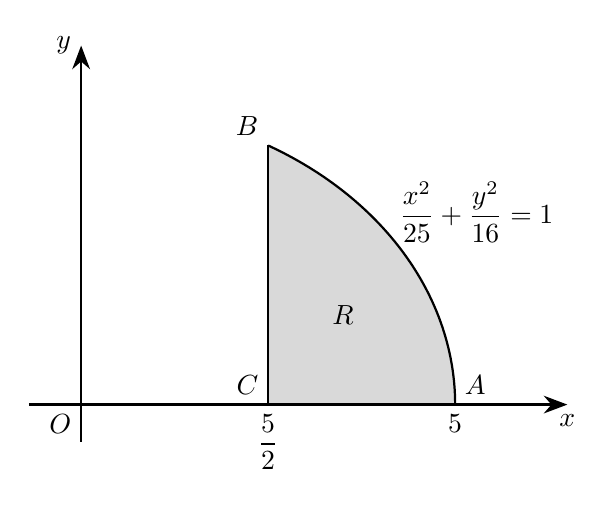
\begin{tikzpicture}[scale=0.95]
\def\a{5}
\def\b{4}
\def\cutfrac{0.5}
\pgfmathsetmacro{\xc}{\a*\cutfrac}
\pgfmathsetmacro{\yb}{\b*sqrt(1-\cutfrac^2)}
\pgfmathsetmacro{\endang}{acos(\cutfrac)}
\coordinate (O) at (0,0);
\coordinate (C) at (\xc,0);
\coordinate (A) at (\a,0);
\coordinate (B) at (\xc,\yb);
\coordinate (E) at ({\a*cos(40)},{\b*sin(40)});
\fill[gray!30] (C) -- (A) -- plot[domain=0:\endang,samples=100] ({\a*cos(\x)},{\b*sin(\x)}) -- cycle;
\draw[thick,black,-{Stealth[length=3mm]}] ({-0.14*\a},0) -- ({1.3*\a},0) node[below] {$x$};
\draw[thick,black,-{Stealth[length=3mm]}] (0,{-0.125*\b}) -- (0,{1.2*\b}) node[left] {$y$};
\draw[thick,black] (C) -- (B);
\draw[thick,black] plot[domain=0:\endang,samples=100] ({\a*cos(\x)},{\b*sin(\x)});
\node[below left] at (O) {$O$};
\node[above left] at (C) {$C$};
\node[below] at (C) {$\dfrac{5}{2}$};
\node[above right] at (A) {$A$};
\node[below] at (A) {$5$};
\node[above left] at (B) {$B$};
\node[right=8pt] at (E) {$\dfrac{x^2}{25}+\dfrac{y^2}{16}=1$};
\node at ($(C)!0.4!(A)+(0,{0.3*\b})$) {$R$};
\end{tikzpicture}
\end{figure}


A uniform lamina occupies the shaded region $R$, bounded by the upper arc of the ellipse
\[
\dfrac{x^2}{25}+\dfrac{y^2}{16}=1
\] \\
the line $x=\frac{5}{2}$ and the $x$-axis. \\

The points $C$ and $A$ have coordinates $\left(\frac{5}{2},0\right)$ and $(5,0)$ respectively. \\
The point $B$ is the upper intersection of the ellipse with $x=\frac{5}{2}$. \\
The unit of length on each axis is one metre. \\
\begin{enumerate}[label=\textbf{(\alph*)}]
\item Using the substitution $x=5\sin t$, show by integration that the area of $R$ is
\[
\dfrac{5}{6}\left(4\pi-3\sqrt{3}\right)\,\mathrm{m}^2
\] \marks[-30pt]{4}
\item Use integration to find the exact coordinates $(\bar{x},\bar{y})$ of the centre of mass of the lamina. \marks{6} \\
\item The lamina is freely suspended from $A$ and hangs in equilibrium. Find the acute angle between $AC$ and the downward vertical, giving your answer in degrees to one decimal place. \marks{3} \\
\end{enumerate}

\newpage

% ---- Question 9 ----
\questionitem
% [Source: _QBT__Centre_of_Mass_of_Laminae_by_Integration, Q9]

\begin{figure}[H]
    \centering
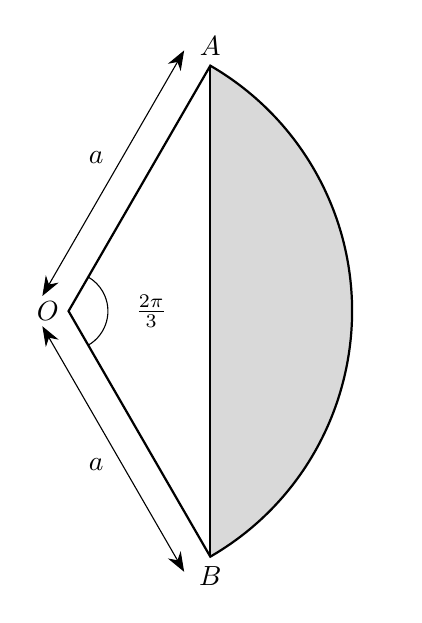
\begin{tikzpicture}[scale=1.2]
\def\rad{3}
\def\ang{60}
\def\dimoff{0.32}
\coordinate (O) at (0,0);
\coordinate (A) at (\ang:\rad);
\coordinate (B) at (-\ang:\rad);
\coordinate (OAstart) at ($(O)+({\ang+90}:\dimoff)$);
\coordinate (OAend) at ($(A)+({\ang+90}:\dimoff)$);
\coordinate (OBstart) at ($(O)+({-\ang-90}:\dimoff)$);
\coordinate (OBend) at ($(B)+({-\ang-90}:\dimoff)$);
\fill[gray!30] (B) arc[start angle=-\ang,end angle=\ang,radius=\rad] -- cycle;
\draw[thick,black] (O) -- (B) arc[start angle=-\ang,end angle=\ang,radius=\rad] -- cycle;
\draw[thick,black] (A) -- (B);
\pic["$\frac{2\pi}{3}$",draw,angle radius=5mm,angle eccentricity=2.1] {angle=B--O--A};
\draw[{Stealth[length=2.5mm]}-{Stealth[length=2.5mm]},black] (OAstart) -- (OAend) node[midway,above left] {$a$};
\draw[{Stealth[length=2.5mm]}-{Stealth[length=2.5mm]},black] (OBstart) -- (OBend) node[midway,below left] {$a$};
\node[left] at (O) {$O$};
\node[above] at (A) {$A$};
\node[below] at (B) {$B$};
\end{tikzpicture}
\end{figure}


A thin uniform metal plate has the shape of the shaded circular segment in the diagram above. \\
It is bounded by the chord $AB$ and the minor arc $AB$ of a circle with centre $O$ and radius $a$, where $a>0$. \\
The angle $AOB$ is $\frac{2\pi}{3}$. \\

The plate is modelled as a uniform lamina with constant mass per unit area $\sigma$, where $\sigma>0$. \\

Take $O$ as the origin and the positive $x$-axis along the bisector of angle $AOB$, directed towards the minor arc. \\
Thus the chord $AB$ lies on $x=\frac{a}{2}$. \\
\begin{enumerate}[label=\textbf{(\alph*)}]
\item Using integration, find the mass of the plate in terms of $\sigma$ and $a$. Give your answer in exact form. \marks{5} \\
\item Using integration to calculate the first moment of the plate about the $y$-axis, find the exact distance of its centre of mass from $O$. Explain why the centre of mass lies on the $x$-axis. \marks{5} \\
\end{enumerate}

\newpage

% ---- Question 10 ----
\questionitem
% [Source: _QBT__Centre_of_Mass_of_Laminae_by_Integration, Q10]

\begin{figure}[H]
    \centering
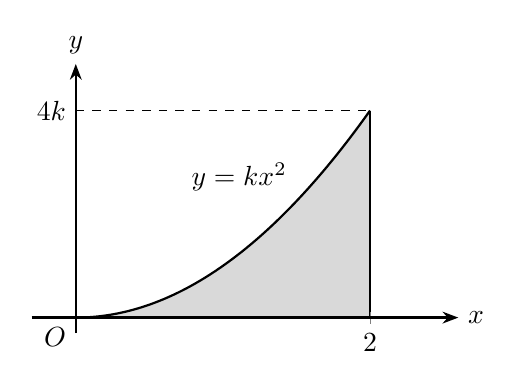
\begin{tikzpicture}
\def\k{1}
\def\extent{2}
\pgfmathsetmacro{\topheight}{\k*\extent^2}
\begin{axis}[axis lines=center,axis line style={thick,black,-{Stealth[length=2mm]}},xmin=-0.3,xmax=2.6,ymin=-0.3,ymax=4.9,width=7cm,height=5cm,xtick={2},ytick=\empty,xlabel={$x$},ylabel={$y$},every axis x label/.style={at={(ticklabel* cs:1)},anchor=west},every axis y label/.style={at={(ticklabel* cs:1)},anchor=south},axis on top,clip=true,clip mode=individual]
\addplot[draw=none,fill=gray!30,domain=0:\extent,samples=100] {\k*x^2} \closedcycle;
\addplot[thick,black,domain=0:\extent,samples=100] {\k*x^2};
\draw[thick,black] (axis cs:\extent,0) -- (axis cs:\extent,\topheight);
\draw[dashed,black] (axis cs:0,\topheight) -- (axis cs:\extent,\topheight);
\node[left] at (axis cs:0,\topheight) {$4k$};
\node[below left] at (axis cs:0,0) {$O$};
\node[above left] at (axis cs:1.5,{\k*1.5^2}) {$y=kx^2$};
\end{axis}
\end{tikzpicture}
\end{figure}


\begin{figure}[H]
    \centering
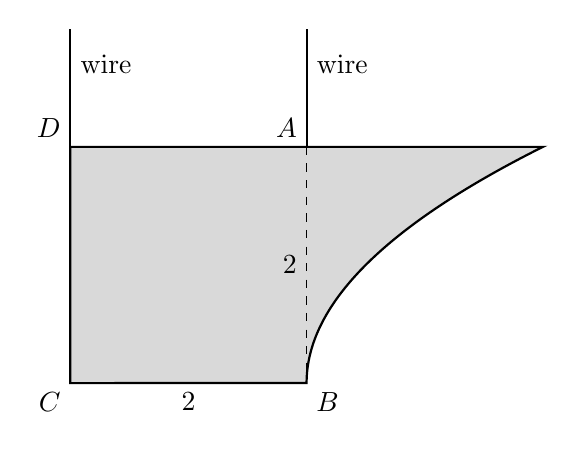
\begin{tikzpicture}[scale=1.5]
\def\k{0.5}
\def\width{2}
\def\height{2}
\def\wirelen{1.0}
\coordinate (C) at (0,0);
\coordinate (B) at (\width,0);
\coordinate (A) at (\width,\height);
\coordinate (D) at (0,\height);
\coordinate (E) at ({\width+\k*\height^2},\height);
\fill[gray!30] (D) -- (E) -- plot[domain=\height:0,samples=100,variable=\t] ({\width+\k*\t^2},\t) -- (C) -- cycle;
\draw[thick,black] (D) -- (E) -- plot[domain=\height:0,samples=100,variable=\t] ({\width+\k*\t^2},\t) -- (C) -- cycle;
\draw[dashed,black] (A) -- (B);
\foreach \P in {A,D} {
  \draw[thick,black] (\P) -- ++(0,\wirelen) node[pos=0.7,right] {wire};
}
\path (A) -- (B) node[midway,left] {$2$};
\path (C) -- (B) node[midway,below] {$2$};
\node[above left] at (A) {$A$};
\node[below right] at (B) {$B$};
\node[below left] at (C) {$C$};
\node[above left] at (D) {$D$};
\end{tikzpicture}
\end{figure}


A uniform lamina occupies the region bounded by the curve $y=kx^2$, the $x$-axis and the line $x=2$, where $k>0$, as shown in the first diagram above. \\
\begin{enumerate}[label=\textbf{(\roman*)}]
\item Use integration to find both coordinates of the centre of mass of this lamina in terms of $k$. \marks{8} \\
\end{enumerate}
A sign is made from a uniform sheet by joining a square $ABCD$ of side length $2$ to a curved piece having the shape of the lamina in part (i). \\
The sheet has the same thickness and density throughout. \\

For the sign, take $C$ as the origin, with $CB$ along the positive $x$-axis and $CD$ along the positive $y$-axis. \\
Thus $A=(2,2)$, $B=(2,0)$ and $D=(0,2)$. \\
The curved piece is obtained by reflecting the lamina in part (i) in the line $y=x$ and then translating it $2$ units to the right. \\
Its curved edge therefore has equation
\[
x=2+ky^2,\qquad 0\leq y\leq2
\] \\
The complete sign is shown in the second diagram above. \\
\begin{enumerate}[label=\textbf{(\roman*)}, resume]
\item Find both coordinates of the centre of mass of the sign in terms of $k$. \marks{5} \\
\end{enumerate}
The sign is held in equilibrium in a vertical plane by two vertical wires attached at $A$ and $D$. \\
The tension in the wire at $A$ is twice the tension in the wire at $D$. \\
\begin{enumerate}[label=\textbf{(\roman*)}, resume]
\item Find the exact value of $k$. \marks{5} \\
\end{enumerate}

\end{enumerate}
\end{document}
